\mainsection{\the\numexpr \thechapter + 1 \relax}{Introduction à la programmation}{dd/mm/yyyy}

\section{Traitement automatique des données}
Un algorithme permet de résoudre un problème donné au moyen d'un nombre fini d'opérations élémentaires. L'application manuelle d'un algorithme est une tâche fastidieuse. C'est pourquoi l'ordinateur a été inventé dans le but d'automatiser l'implémentation de l'algorithme. On parle de l'informatique comme \textit{la science de traitement automatique de l'information}.\\

Ce  que l'on attend d'un programme c'est qu'il prenne les données d'entrée du problème, qu'il les transforme au moyen de l'algorithme, et qu'il redonne le résultat attendu.
\begin{center}
	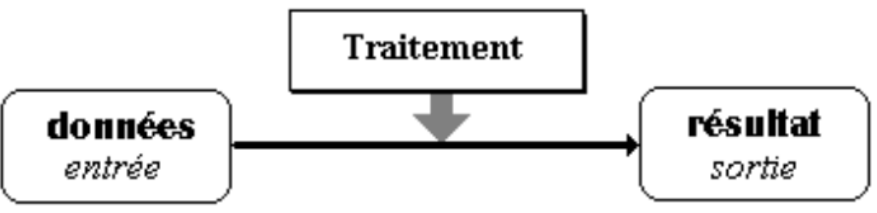
\includegraphics[trim=0 0 0 20,width=0.5\textwidth]{Images/shema_science_info}
\end{center}
Pour que le programme s'exécute sur un ordinateur, il faut indiquer à la machine comment si prendre. 
D'un côté l'ordinateur qui comprend seulement le langage binaire composé d'une suite de 0 et de 1 et de l'autre, le programmeur qui parle un langage destiné à la communication entre humains comme le français rempli d'ambiguïtés (plusieurs interprétations possibles de la même phrase). Il faut trouver un intermédiaire, c'est ce qu'on appelle un \textbf{langage de programmation}. 
\begin{mydefinition}
	Un \textbf{langage de programmation} est un langage formel utilisé pour expliquer en détail à un ordinateur comment réaliser une tâche.
\end{mydefinition}
Les langages de programmation sont caractérisés par une \textbf{syntaxe} très rigide (afin qu'aucune ambiguïté n'existe) et qui permet aux ordinateurs d'exécuter ce que les humains leur disent de faire. La syntaxe de codage sera constituée d'ensembles de mots et symboles spécifiques qui devront se combiner  dans un ordre bien particulier (\textbf{règle de syntaxe}). Chaque fois que cet ordre ne sera pas satisfait, l'ordinateur généra une erreur (\textbf{erreur de syntaxe}).
\begin{mydefinition}
	Les \textbf{règles de syntaxe} définissent l’ensemble des programmes qui sont valides et acceptables par l’interpréteur/compilateur.
	En français, les règles de syntaxe incluent l’orthographe et la grammaire, et déterminent quelles sont les phrases valides.
\end{mydefinition}

\begin{eclairage}
	\textbf{Langages naturels Vs Langages de programmation} 
	\begin{multicols}{2}
		\textbf{Langages naturels}
		\begin{itemize}
			\item Communiquer entre humains
			\item Mots corrects (orthographe)
			\item Phrases correctes (grammaire)
		\end{itemize}
		\newpage
		\textbf{Langages de programmation}
		\begin{itemize}
			\item Indiquer à une machine comment résoudre un problème
			\item Identificateurs valides
			\item Syntaxe valide
		\end{itemize}
	\end{multicols}
\end{eclairage}



\section{Langages de programmation}
Pour que le programme écrit dans un langage de programmation soit compréhensible par l'ordinateur il devra être traduit par un programme appelé interpréteur ou compilateur (en fonction du type de langage et de son application). À l'heure actuelle plusieurs centaines de langages de programmation sont utilisés en fonction du domaine, des applications et des préférences du programmeur.
\begin{center}
	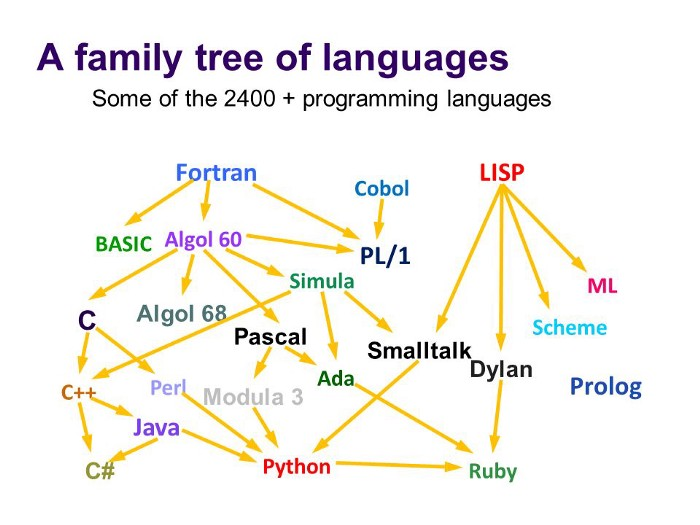
\includegraphics[scale=0.45,trim=0 40 0  160,clip=true]{Images/family_tree_languages}
	\captionof{figure}{Arbre généalogique des langages de programmation les plus utilisés.}
\end{center}
Il existe plusieurs critères pour catégoriser tous ces langages de programmation. Nous allons en passer en revue quelques-uns.

\subsection{Paradigmes de programmation}
Selon Wikipedia, \textit{un \textbf{paradigme de programmation} est une façon d'approcher la programmation informatique et de traiter les solutions aux problèmes et leur formulation dans un langage de programmation approprié}. Les paradigmes les plus communs sont 
\begin{enumerate}
	\itemb{programmation impérative}  
	\itemb{programmation fonctionnelle}
	\itemb{programmation orientée objet}
\end{enumerate}
Certains langages de programmation permettent de programmer en utilisant plusieurs approches. C'est notamment le cas du langage Python que nous utiliserons dans ce cours, même si nous adopterons principalement l'approche impérative.

\subsection{Proximité avec le langage binaire-machine}	
On différencie  des langages de programmation  en fonction de leur proximité avec le langage binaire-machine qui est considérée comme le langage de plus bas niveau. On distingue deux niveaux :
\begin{enumerate}
	\itemb{bas niveau (proche machine) :}  permet de contrôler tout ce qui se passe dans la machine pendant l'exécution du code.\\
	C'est un langage machine lisible par un humain qui permet simplement de  manipuler explicitement des registres, des adresses mémoires, voire des instructions machines.  Par exemple~: assembleur, C\ldots.\\
	
	
	\itemb{haut niveau (proche utilisateur) :}  permet à l'utilisateur d'utiliser des fonctions complexes sans se soucier de l'aspect machine (enfin un petit peu quand même).  Pour son optimisation, il utilise parfois (souvent) des langages de bas niveau de façon transparente pour l'utilisateur.  Par exemple : FORTRAN, Python, PHP, SQlite\ldots
\end{enumerate}

\subsection{Langage interprété et langage compilé}		
On peut aussi trier les langages entre langages de programmation interprétés  et langages de programmation compilés:
\begin{enumerate}
	\itemb{interprété :} le langage est lu avec un programme appelé interpréteur pour exécuter le code au fur et à mesure de la lecture du code.  \\
	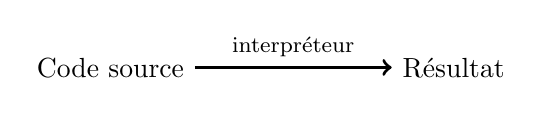
\begin{tikzpicture} 
		\draw [very thick,->](0,0)node[left]{Code source}--node[above]{\footnotesize interpréteur}++(2.5,0)node[right]{Résultat};
	\end{tikzpicture}
	\begin{enumerate}
		\item{avantage :} Test immédiat 
		\item{inconvénient :} plus lent, le code est interprété à chaque lancement du \textbf{programme interprété}.
	\end{enumerate}
	\itemb{compilé :} le langage est converti en langage machine (binaire) par l'intermédiaire d'un programme dédié (compilateur) qui produit un programme qui pourra dorénavant s'exécuter seul.\\
	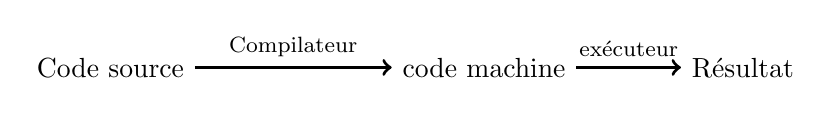
\begin{tikzpicture} 
		\draw [very thick,->](0,0)node[left]{Code source}--node[above]{\footnotesize Compilateur}++(2.5,0)node[right](m){code machine};
		\draw [very thick,->](m)--node[above]{\footnotesize exécuteur}++(2.5,0)node[right](m){Résultat};
	\end{tikzpicture}
	\begin{enumerate}
		\item{avantage :} Rapide
		\item{inconvénient :} nécessite une première étape de compilation.
	\end{enumerate}
\end{enumerate}

\subsection{Langages visuels}		
La rigidité et l'austérité des langages de programmation classique a poussé les programmeurs à développer des langages de programmation visuels qui simplifie l'apprentissage de la programmation. Dans un langage visuel, les éléments du langage de programmation sont accessibles sous la forme d’éléments graphiques (le plus souvent des blocs).
\begin{enumerate}
	\item{avantage :} des symboles clairs et une absence  de syntaxe ->  les erreurs de saisie sont impossibles
	\item{inconvénient :} Manque de modularité, il devient très difficile de structurer le programme pour des projets importants.
\end{enumerate}
\begin{figure}[!h]
	\centering
	\subfloat[Langage visuel]{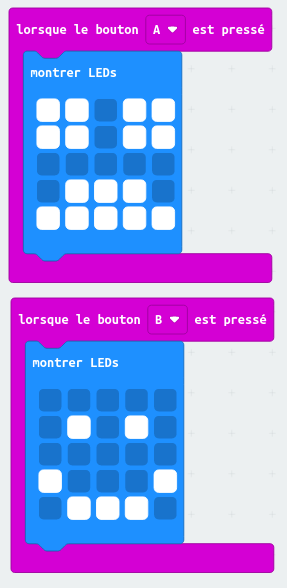
\includegraphics[scale=0.5]{Images/blockly_ex}}
	\hspace{1cm}
	\subfloat[Langage textuel]{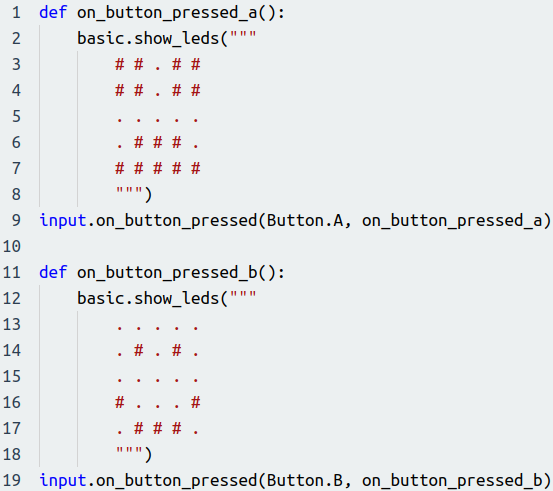
\includegraphics[scale=0.5]{Images/micropython_ex}}
	\caption{Le même programme écrit dans deux langages différents.}
\end{figure}\label{CourbeRepr}


\section{La langage \py et l'IDE Thonny}
\subsection{\py}
Quel est le meilleur langage de programmation? Cette seule question a permis de remplir des centaines de forum de programmeurs sur internet. Chaque langage ayant ses avantages, ses particularités et spécificités liées au matériel et type d'applications à créer. Cette année, nous utiliserons le langage \py. Voici un échantillon de raisons qui ont motivé notre choix \footnote{Voir l'article sur  \url{https://linux-center.org/articles/9812/python.html}}:
\begin{itemize}
	\item \py est un langage interprété ce qui rend le code portable sur la plupart des ordinateurs/systèmes d'exploitation.
	\item La syntaxe de \py est très simple. 
	\item Code lisible et compact
	\item \py est gratuit.
	\item \py est très utilisé, en particulier pour l'apprentissage de la programmation.
	\item \py est en 2021 le langage le plus utilisé dans le monde selon la classification\footnote{Voir la classification sur \url{https://spectrum.ieee.org/top-programming-languages-2021}} IEEE\footnote{IEEE: Institute of Electrical and Electronics Engineers ou en français: l'Institut des ingénieurs électriciens et électroniciens} Spectrum 
	\item etc...
\end{itemize}

\subsection{Environnement de Développement Intégré Thonny}
\py est un langage interprété, donc pour écrire des programmes \py nous aurons besoin d':
\begin{itemize}
	\item un éditeur de texte pour écrire le code;
	\item un interpréteur \py pour tester le code ou des instructions;
	\item éventuellement, un débogueur pour pouvoir exécuter les instructions du programme les unes après les autres afin d'identifier les erreurs de programmations.
\end{itemize}
Un logiciel comme \textbf{Thonny}, intègre ces différents aspects dans un seul logiciel, on appelle ce type de logiciel un  Environnement de  Développement Intégré (IDE en anglais pour \textit{Integrated Development Environment}),
\begin{figure}[!h]
	\centering
	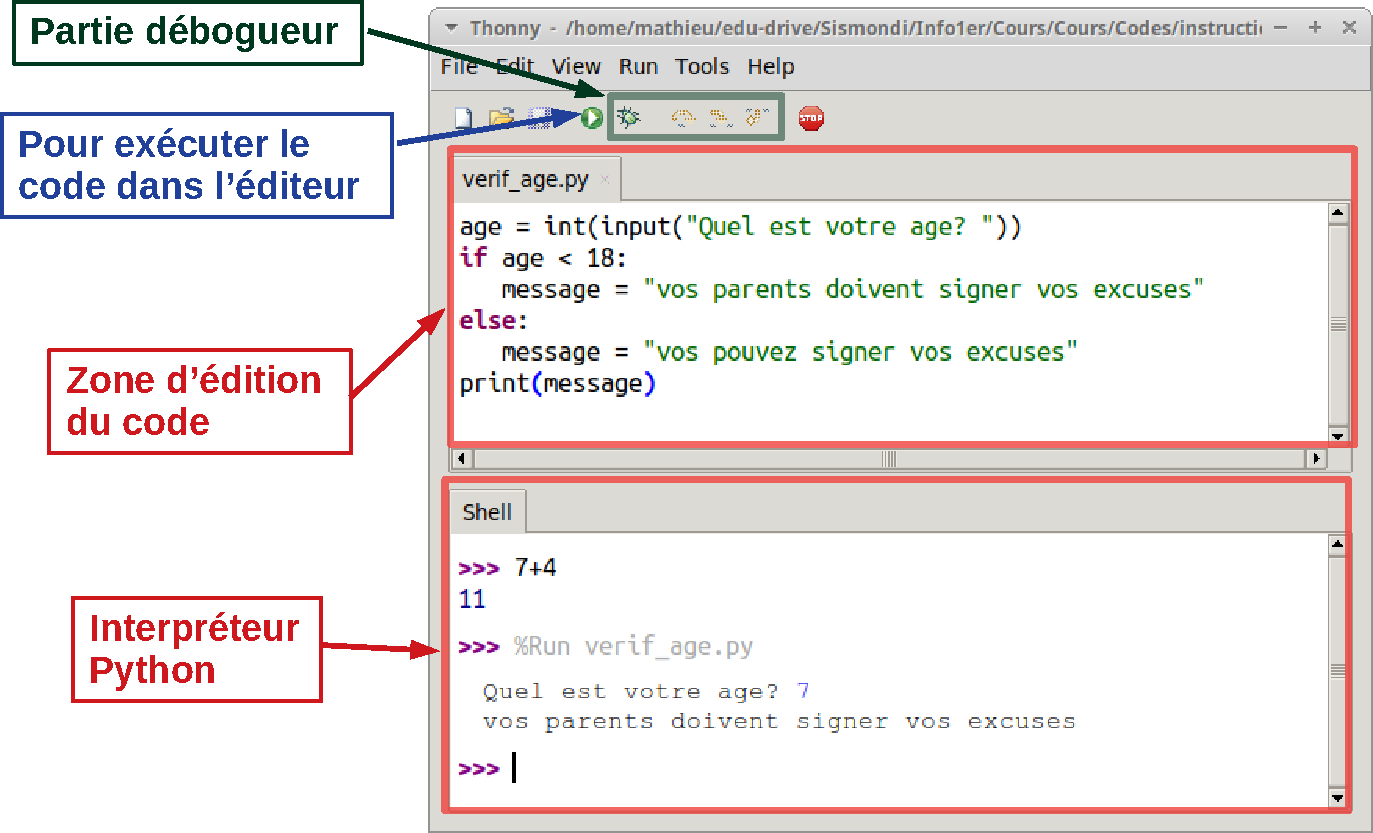
\includegraphics[scale=0.5]{Images/IDE_Thonny_illustre-crop.pdf}
	\caption{IDE Thonny}
\end{figure}
\subsubsection{Interpréteur \py}
L'interpréteur \py se présente sous la forme d’une fenêtre avec des \lstinline{>>>} après lesquels on peut entrer des instructions. En pressant la touche \textit{Entrée} du clavier, \py interprète les instructions et affiche le résultat.

\subsubsection{L'éditeur}
Lorsque l'on souhaite taper une suite de commandes, on préfère créer un script (programme) avec l'éditeur. Ainsi on peut sauvegarder son travail dans un fichier texte. Pour exécuter le code tapé dans l'éditeur, il suffit de cliquer sur le bouton vert avec la pointe de flèche.
\begin{important}
	On utilisera l'extension .py pour enregistrer les fichiers qui contiennent du code \py. De plus, on veillera à utiliser un nom de fichier cours mais explicatif sans utiliser d'accent et d'espace (les espaces peuvent être remplacer par le caractère \_ \textit{underscore})
\end{important}


\subsection{Première rencontre avec un programme Python}
Dans un langage impératif, un programme est constitué d'instructions qui vont de la première à la dernière lignes. Comme nous le verrons pas la suite, l'ordre d'exécution entre la première et la dernière instruction pourra varier en fonction d'instructions de contrôle de flux. Prenons le programme, écrit en \py, suivant:

\vspace{-0.7cm}
\begin{monprogramme}
	\lstinputlisting[label={premierprg}, caption=Premier programme Python ]
	{Codes/into_lang_prog/premier_prog_python.py}
\end{monprogramme}
%
\begin{question}
	Que fait ce programme?
\end{question}


\begin{eclairage}
	Le but d'un programme est de traiter de l'information en entrée afin de produire le résultat attendu en sortie. Par conséquent, on retrouvera souvent la structure suivante:
	\begin{itemize}
		\item Une partie entrée où les données du problème sont obtenus (lignes 2 à 5 dans le programme \ref{premierprg}).
		\item Le corps du programme où un algorithme est exécuté instruction après instruction en fonction des données lues (lignes 7 à 13 dans le programme \ref{premierprg});
		\item Une partie sortie qui affiche ou stocke le résultat obtenu (ligne 15 dans le programme \ref{premierprg}).
	\end{itemize}
	Nous verrons par la suite qu'un programme est essentiellement constitué d’expressions ou structures de données et d’instructions ou structures de contrôles. Il contiendra toujours les 4 ingrédients de base suivants
	\begin{itemize}
		\itemb{des structure de données} : les variables (qui représenteront l’Information).
		\itemb{3 types de structures de contrôle du flux d’instructions} (qui permettront de traiter cette Information) :
		\begin{itemize}
			\item Les séquences d’instructions.
			\item Les tests conditionnels ou alternatives.
			\item Les boucles ou répétitions.
		\end{itemize}
	\end{itemize}
\end{eclairage}
